\chapter{Projekt aplikacji}
\thispagestyle{chapterBeginStyle}
\label{rozdzial2}
W tym rozdziale przedstawiono szczegółowy projekt systemu korzystając z notacji UML oraz uwzględniając założenia funkcjonalne z rozdziału \ref{wstep}.
Scharakteryzowano przypadki użycia oraz towarzyszące im scenariusze. Przedstawiono ogólną strukturę aplikacji w diagramie komponentów. Określono tryby działania aplikacji poprzez diagram stanów. Przedstawiono projekt bazy danych. Opisano dokładnie protokół komunikacji z MiBandem 3. 

\section{Przypadki użycia}
Poniżej przedstawiono ogólny diagram przypadków użycia \ref{use_case}. Szczegółowe scenariusze zostały zdefiniowane w odpowiednich podsekcjach tego podrozdziału.
\begin{figure}[H]
    \begin{center}
        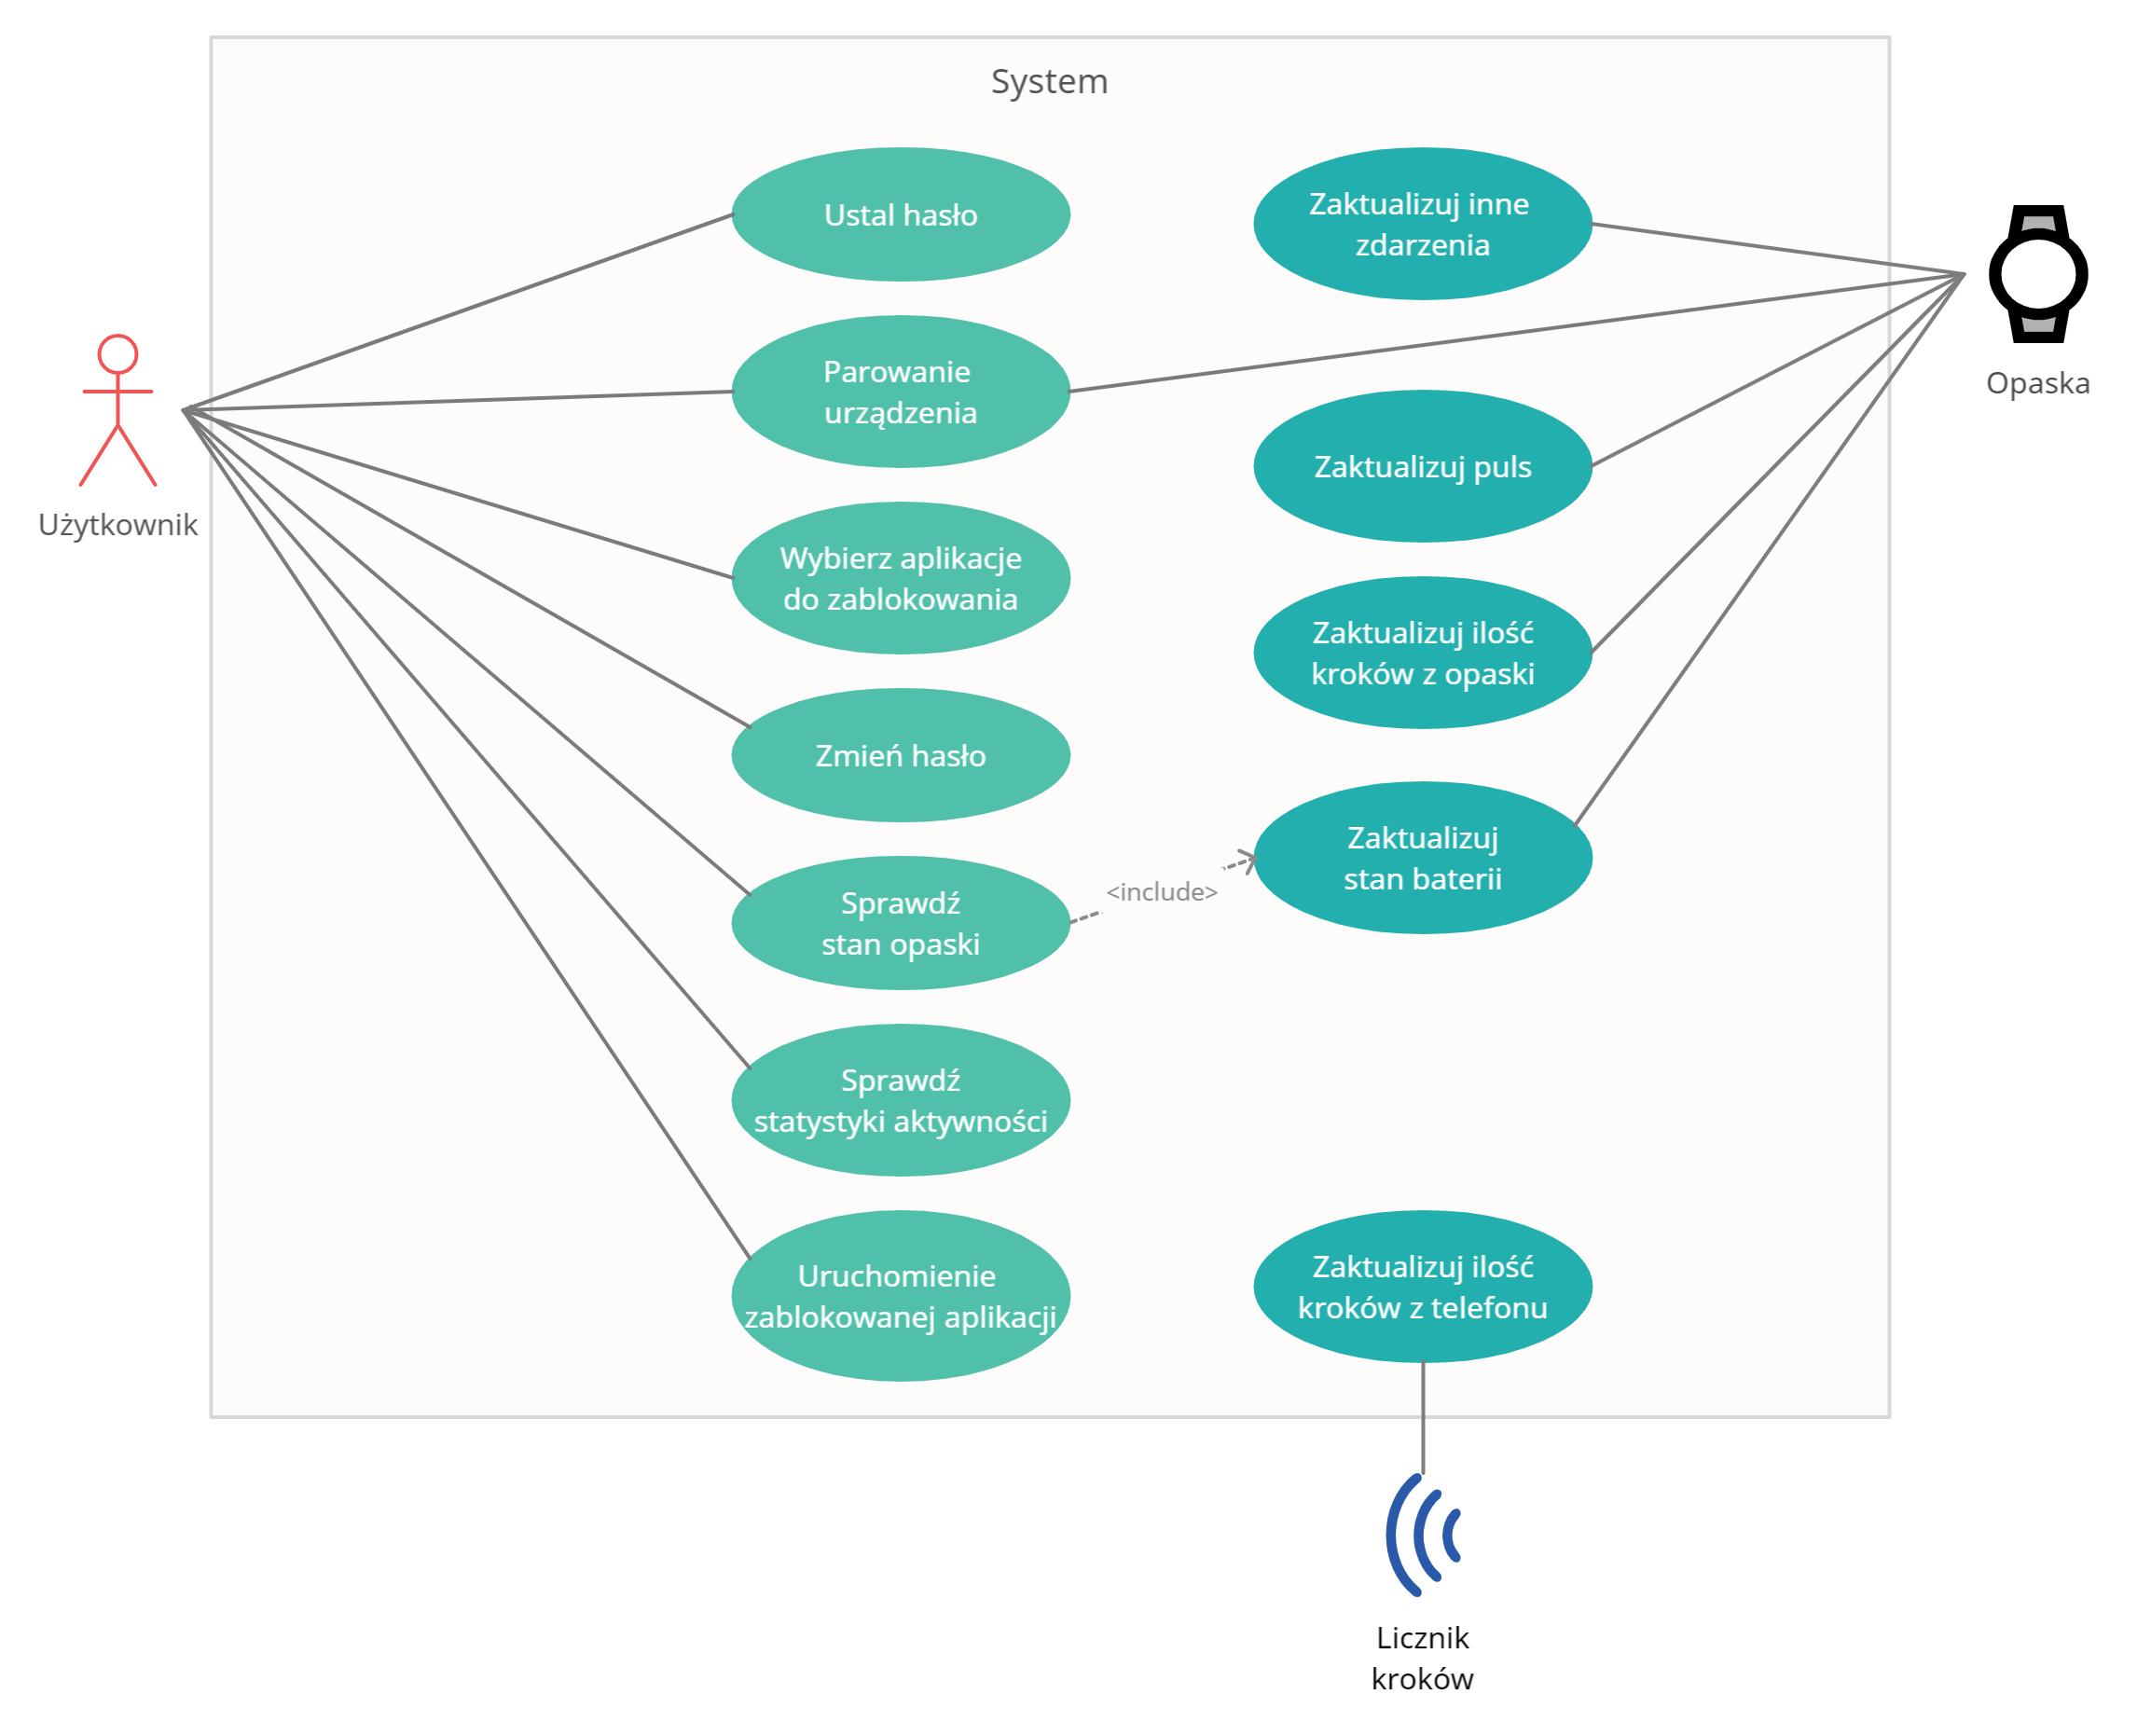
\includegraphics[width=0.9\textwidth]{UseCaseDiagram.png}
    \end{center}
    \caption{{\color{dgray}Diagram przypadków użycia.}} \label{use_case}
\end{figure}

\subsection{Ustal hasło}
W tym przypadku użytkownik aplikacji ustala hasło, które jest potrzebne przy odblokowywaniu dostępu do zablokowanych aplikacji. Aktorami są Użytkownik oraz System. Obecny przypadek użycia jest inicjowany przy pierwszym uruchomieniu aplikacji, kiedy nie istnieje jeszcze zaszyfrowany plik, w którym będzie przechowywane hasło. Po wykonaniu przypadku w systemie zostaje zarejestrowane hasło użytkownika, które będzie później wykorzystane w celu dezaktywacji blokady aplikacji. Scenariusz składa się z następującego przepływu głównego:
\begin{enumerate}
    \item Aplikacja wyświetla formularz zawierający pola Hasło oraz Powtórz hasło.
    \item Użytkownik wprowadza identyczne hasła do podanych pól oraz zatwierdza wprowadzone dane przyciskiem znajdującym się poniżej.
    \item System sprawdza zgodność haseł oraz czy spełniają wymagane kryteria.
    \item System tworzy zaszyfrowany plik i zapisuje w nim hasz hasła.
\end{enumerate}
Alternatywnie:
\newline\newline
\indent 3. Jeśli wprowadzone hasła nie są zgodne:
\begin{enumerate}[leftmargin=3\parindent]
    \item Zostaje wyświetlony komunikat o błędzie.
    \item Następuje powrót do kroku numer 2 w głównym przepływie.
\end{enumerate}

\subsection{Parowanie urządzenia}
W tym przypadku użytkownik aplikacji skanuje otoczenie, korzystając z modułu Bluetooth w poszukiwaniu najbliższej opaski MiBand, a następnie nawiązuje z nią pierwsze połączenie. Aktorami są Użytkownik, System oraz Opaska. Przypadek ten występuje przy pierwszym uruchomieniu systemu, kiedy zostało już ustalone hasło odblokowujące. Po zakończeniu system jest sparowany z opaską MiBand, z którą komunikacja jest kluczowym punktem działania systemu. W systemie zostaje także zapisany adres MAC opaski, dzięki czemu będzie można z łatwością ponownie połączyć się z nią. Główny przepływ składa się z następujących kroków:
\begin{enumerate}
    \item Użytkownik naciska przycisk ``Skan''.
    \item System rozpoczyna skanowanie urządzeń Bluetooth Low Energy w celu znalezienia Opaski.
    \item System wyświetla znalezione Opaski w formie listy. 
    \item Użytkownik wybiera Opaskę, do której się podłączy poprzez naciśnięcie na jej nazwę.
    \item System tworzy więź z wybraną Opaską i inicjuje pierwsze połączenie.
\end{enumerate}
Alternatywnie:
\newline\newline
\indent 3. Jeśli nie znaleziono żadnej Opaski:
\begin{enumerate}[leftmargin=3\parindent]
    \item Zostaje wyświetlony komunikat o błędzie.
    \item Następuje powrót do kroku numer 1 w głównym przepływie.
\end{enumerate}
\quad\newline
\indent 5. Jeśli wystąpi błąd połączenia z Opaską:
\begin{enumerate}[leftmargin=3\parindent]
    \item Następuje powrót do kroku numer 4 w głównym przepływie.
\end{enumerate}

\subsection{Wybierz aplikacje do zablokowania}
W tym przypadku użytkownik aplikacji wybiera z listy zainstalowanych aplikacji te, które będą blokowane przez system kiedy zostanie uruchomiona blokada. Aktorami są Użytkownik oraz System. Przypadek ten występuje, gdy istnieje plik z hasłem, opaska została sparowana, nie ma uruchomionej blokady oraz Użytkownik uruchomił aplikację. Po zakończeniu System posiada informację, na których aplikacjach uruchamiać blokadę. Główny przepływ składa się z następujących kroków:
\begin{enumerate}
    \item Użytkownik z poziomu głównego ekranu aplikacji przechodzi do Ustawień.
    \item Użytkownik wybiera opcję Zablokowane aplikacje.
    \item Użytkownik zaznacza aplikację z listy, którą chce zablokować bądź odblokować.
    \item System zapisuje aktualny stan aplikacji.
\end{enumerate}

\subsection{Zmień hasło}
W tym przypadku użytkownik aplikacji zmienia hasło odblokowujące dostęp do zablokowanych aplikacji. Aktorami są Użytkownik oraz System. Przypadek ten występuje, gdy istnieje plik z hasłem, opaska została sparowana, nie ma uruchomionej blokady oraz Użytkownik uruchomił aplikację. Po zakończeniu System posiada informację o nowym haśle, które będzie wykorzystywane od tej pory do odblokowywania dostępu. Główny przepływ składa się z następujących kroków:
\begin{enumerate}
    \item Użytkownik z poziomu głównego ekranu aplikacji wybiera opcję Ustawienia w dolnej nawigacji.
    \item Użytkownik wybiera opcję Zmień hasło.
    \item Użytkownik wpisuje odpowiednie wartości do pól Stare hasło, Nowe hasło oraz Powtórz nowe hasło oraz zatwierdza wprowadzone dane.
    \item System zapisuje hasz nowego hasła w zaszyfrowanym pliku.
\end{enumerate}
Alternatywnie: 
\newline\newline
\indent 3. Jeśli stare hasło jest błędne lub nowe hasło nie zgadza się z powtórzonym:
\begin{enumerate}[leftmargin=3\parindent]
    \item System wyświetla komunikat o błędnych wprowadzonych danych.
    \item Następuje powrót do kroku numer 3 w głównym przepływie.
\end{enumerate}
\quad\newline
\indent 4. Jeśli wystąpi błąd zapisu:
\begin{enumerate}[leftmargin=3\parindent]
    \item System wyświetla komunikat o błędzie zapisu.
    \item Następuje powrót do kroku numer 3 w głównym przepływie.
\end{enumerate}

\subsection{Sprawdź stan opaski}
W tym przypadku użytkownik aplikacji sprawdza podstawowe informacje na temat opaski oraz jej stan baterii. Aktorami są Użytkownik, System oraz Opaska. Przypadek ten występuje, gdy istnieje plik z hasłem, opaska została sparowana, nie ma uruchomionej blokady oraz Użytkownik uruchomił aplikację. Po zakończeniu Użytkownik zna stan baterii oraz inne informacje o Opasce, a System zyskuje odświeżony stan baterii Opaski. Głowny przepływ składa się z następujących kroków:
\begin{enumerate}
    \item Użytkownik z poziomu głównego ekranu aplikacji wybiera opcję Opaska w dolnej nawigacji.
    \item System wyświetla zapisane wcześniej informacje o Opasce.
    \item Przejdź do przypadku Zaktualizuj stan baterii
    \item System aktualizuje wartość baterii na ekranie.
\end{enumerate}
Alternatywnie:
\newline\newline
\indent 2. Jeśli nie zapisano wcześniej informacji o Opasce:
\begin{enumerate}[leftmargin=3\parindent]
    \item System wyświetla w brakujących polach wartość Nieznane.
    \item Następuje przejście do kroku numer 3 w głównym przepływie.
\end{enumerate}
\quad\newline
\indent 3. Jeśli nastąpi nagła utrata połączenia z Opaską:
\begin{enumerate}[leftmargin=3\parindent]
    \item Pomiń następny krok w głównym przepływie.
\end{enumerate}

\subsection{Sprawdź statystyki aktywności}
W tym przypadku użytkownik aplikacji sprawdza proste statystyki zarejestrowanej dziennej aktywności. Aktorami są Użytkownik oraz System. Przypadek ten występuje, gdy istnieje plik z hasłem, opaska została sparowana, nie ma uruchomionej blokady oraz Użytkownik uruchomił aplikację. Po zakończeniu Użytkownik zna ilość zarejestrowanych kroków oraz ostatnią zarejestrowaną wartość pulsu. Główny przepływ składa się z następujących kroków:
\begin{enumerate}
    \item Użytkownik z poziomu głównego ekranu aplikacji wybiera opcję Statystyki w dolnej nawigacji.
    \item System wyświetla ostatnie zapisane wartości dziennych kroków oraz pulsu.
    \item System aktualizuje wyświetlane wartości, gdy zostaną zapisane nowe.
\end{enumerate}

\subsection{Uruchomienie zablokowanej aplikacji}
W tym przypadku użytkownik aplikacji próbuje uruchomić aplikację z listy zablokowanych podczas, gdy uruchomiona jest blokada. Aktorami są Użytkownik i System. Przypadek ten występuje, gdy istnieje plik z hasłem, opaska została sparowana oraz aplikacja pracuje w trybie blokady. Po zakończeniu Użytkownik posiada autoryzację do interakcji z blokowanymi aplikacjami, a System przechodzi w tryb monitorowania. Główny przepływ składa się z następujących kroków:
\begin{enumerate}
    \item Użytkownik uruchamia aplikację z listy zablokowanych.
    \item System przenosi Użytkownika w ekran wprowadzania hasła.
    \item Użytkownik wprowadza hasło i zatwierdza.
    \item System wyłącza blokadę i uruchamia usługę monitorującą.
\end{enumerate}
Alternatywnie:
\newline\newline
\indent 3. Jeśli Użytkownik wprowadził błędne hasło:
\begin{enumerate}[leftmargin=3\parindent]
    \item System wyświetla komunikat o błędnym haśle.
    \item Następuje ponowne wykonanie kroku 3 z głównego przepływu.
\end{enumerate}

\subsection{Zaktualizuj inne zdarzenia}
W tym przypadku opaska rejestruje jedno z podejrzanych zdarzeń i przesyła informację o tym do aplikacji. Aktorami są Opaska oraz System. Przypadek ten występuje, gdy istnieje plik z hasłem, opaska została sparowana i jest aktywne połączenie między nią a aplikacją. Po zakończeniu System zyskuje sygnał do uruchomienia blokady. Główny przepływ składa się z następujących kroków:
\begin{enumerate}
    \item Opaska rejestruje jedno z zaprogramowanych zdarzeń.
    \item Opaska przesyła kod zdarzenia do Systemu.
    \item System porównuje otrzymany kod z zapisanymi kodami podejrzanych zdarzeń.
    \item System uruchamia blokadę.
\end{enumerate}
Alternatywnie:
\newline\newline
\indent 2. Jeśli nastąpi nagła utrata połączenia:
\begin{enumerate}[leftmargin=3\parindent]
    \item Następuje przejście do kroku numer 4 w głównym przepływie.
\end{enumerate}
\quad\newline
\indent 3. Jeśli otrzymany kod nie znajduje się na liście podejrzanych:
\begin{enumerate}[leftmargin=3\parindent]
    \item Pomiń następny krok głównego przepływu.
\end{enumerate}
\subsection{Zaktualizuj puls}
W tym przypadku opaska wykonuje automatyczny pomiar pulsu i przesyła jego wartość do aplikacji. Aktorami są Opaska oraz System. Przypadek ten występuje, gdy istnieje plik z hasłem, opaska została sparowana i jest aktywne połączenie między nią a aplikacją. Po zakończeniu System zyskuje aktualne dane na temat pulsu do analizy stanu użytkownika. Główny przepływ składa się z następujących kroków:
\begin{enumerate}
    \item Opaska mierzy puls.
    \item Opaska przesyła zarejestrowaną wartość do Systemu.
    \item System zapisuje otrzymaną wartość.
\end{enumerate}
Alternatywnie:
\newline\newline
\indent 2. Jeśli nastąpi nagła utrata połączenia:
\begin{enumerate}[leftmargin=3\parindent]
    \item System uruchamia blokadę.
\end{enumerate}
\quad\newline
\indent 3. Jeśli otrzymana wartość wynosi 0:
\begin{enumerate}[leftmargin=3\parindent]
    \item System uruchamia blokadę.
\end{enumerate}

\subsection{Zaktualizuj ilość kroków z opaski}
W tym przypadku opaska rejestruje wykonane kroki oraz przesyła uaktualnioną wartość dziennych wykonanych kroków do aplikacji. Aktorami są Opaska oraz System. Przypadek ten występuje, gdy istnieje plik z hasłem, opaska została sparowana i jest aktywne połączenie między nią a aplikacją. Po zakończeniu System zyskuje aktualne dane na temat wykonanych kroków, które zostaną wykorzystane później do analizy zachowania użytkownika. Główny przepływ składa się z następujących kroków:
\begin{enumerate}
    \item Opaska rejestruje wykonanie kroków.
    \item Opaska przesyła zaktualizowaną wartość dziennych kroków do Systemu.
    \item System zapisuje otrzymaną wartość.
\end{enumerate}
Alternatywnie:
\newline\newline
\indent 2. Jeśli nastąpi nagła utrata połączenia:
\begin{enumerate}[leftmargin=3\parindent]
    \item System uruchamia blokadę.
\end{enumerate}
\quad\newline
\indent 3. Jeśli otrzymana wartość jest równa ostatniemu pomiarowi:
\begin{enumerate}[leftmargin=3\parindent]
    \item System nie zapisuje otrzymanej wartości.
\end{enumerate}

\subsection{Zaktualizuj stan baterii}
W tym przypadku aplikacja odczytuje aktualny stan baterii z opaski. Aktorami są Opaska oraz System. Przypadek ten występuje, gdy istnieje plik z hasłem, opaska została sparowana i jest aktywne połączenie między nią a aplikacją. Po zakończeniu System zyskuje aktualną wartość stanu baterii. Główny przepływ składa się z następujących kroków:
\begin{enumerate}
    \item System przesyła do Opaski zapytanie o stan baterii.
    \item Opaska przesyła do Systemu aktualny stan baterii.
    \item System zapisuje nową wartość stanu baterii.
\end{enumerate}
Alternatywnie:
\newline\newline
\indent 2. Jeśli nastąpi nagła utrata połączenia:
\begin{enumerate}[leftmargin=3\parindent]
    \item System uruchamia blokadę.
\end{enumerate}

\subsection{Zaktualizuj ilość kroków z telefonu}
W tym przypadku sensor licznika kroków w smartfonie rejestruje wykonane kroki, a następnie informuje aplikację o aktualizacji swojej wartości. Aktorami są Licznik kroków oraz System. Przypadek ten występuje, gdy istnieje plik z hasłem, opaska została sparowana i jest aktywna usługa monitorująca zachowanie użytkownika. Po zakończeniu System zyskuje informację na temat wykonanych kroków, która zostanie później wykorzystana do analizy zachowania użytkownika.
\begin{enumerate}
    \item Licznik kroków rejestruje wykonanie kroków.
    \item System odczytuje zaktualizowaną liczbę kroków Licznika kroków.
    \item System zapisuje odczytaną wartość.
\end{enumerate}

\section{Diagram pakietów}

W tej sekcji należy przedstawić diagramy komponentów dla odpowiednich elementów systemu zidentyfikowane na podstawie wcześniejszych rozważań

\section{Diagram stanów}

Na grafice \ref{main_state_diagram} przedstawiono diagram stanów dla systemu monotorująco-blokującego, stanowiącego podstawę działania aplikacji. Diagram ten przedstawia ogólny schemat działania aplikacji w zakresie zabezpieczenia smartfona. Stanami początkowymi są \textit{Zakończono początkową konfigurację} oraz \textit{Uruchomiono ponownie system}. Przedstawiają one dwie sytuacje, w których może nastąpić uruchomienie systemu. W pierwszym przypadku jest to pierwsze uruchomienie aplikacji, gdzie określono hasło i nawiązano połączenie z opaską. Wtedy następuje przejście do stanu \textit{Monitorowanie aktywności}. W przypadku restartu urządzenia wybór stanu, do którego przejdzie aplikacja zależy od ostatniego aktywnego stanu przed wyłączeniem urządzenia. Jeśli była aktywna blokada, aplikacja przejdzie do stanu \textit{Monitorowanie otwieranych aplikacji}. W przeciwnym razie przejdzie do stanu \textit{Łączenie z opaską}.
\newline\newline
\indent Następnym analizowanym stanem jest \textit{Monitorowanie aktywności}. W tym stanie aplikacja pobiera dane z opaski i analizuje je pod kątem zdarzeń sugerujących, że użytkownik nie nadzoruje swojego smartfona. Jeśli zostanie wykryte takie zdarzenie następuje przejście do kolejnego analizowanego stanu - \textit{Monitorowanie otwieranych aplikacji}. W tym stanie system skanuje statystyki użycia innych aplikacji w krótkich odstępach czasu. Jeśli zostanie wykryte przejście do aplikacji na liście zablokowanych następuje przejście do stanu \textit{Oczekiwanie na wprowadzenie hasła}. W tym stanie aplikacja wyświetla okno wprowadzania hasła i czeka na akcje użytkownika. Możliwe są trzy przejścia: gdy użytkownik zamknie okno aplikacja powraca do stanu \textit{Monitorowanie otwieranych aplikacji}, gdy wprowadzone hasło jest błędne system pozostaje w tym samym stanie, a gdy wprowadzone zostanie poprawne hasło system przechodzi do stanu \textit{Łączenie z opaską}. W tym stanie aplikacja próbuje nawiązać połączenie z opaską. Gdy zakończy się to sukcesem zachodzi przejście do stanu \textit{Monitorowanie aktywności}. W przeciwnym razie aplikacja powraca do stanu \textit{Monitorowanie otwieranych aplikacji}.

\begin{figure}[H]
    \begin{center}
        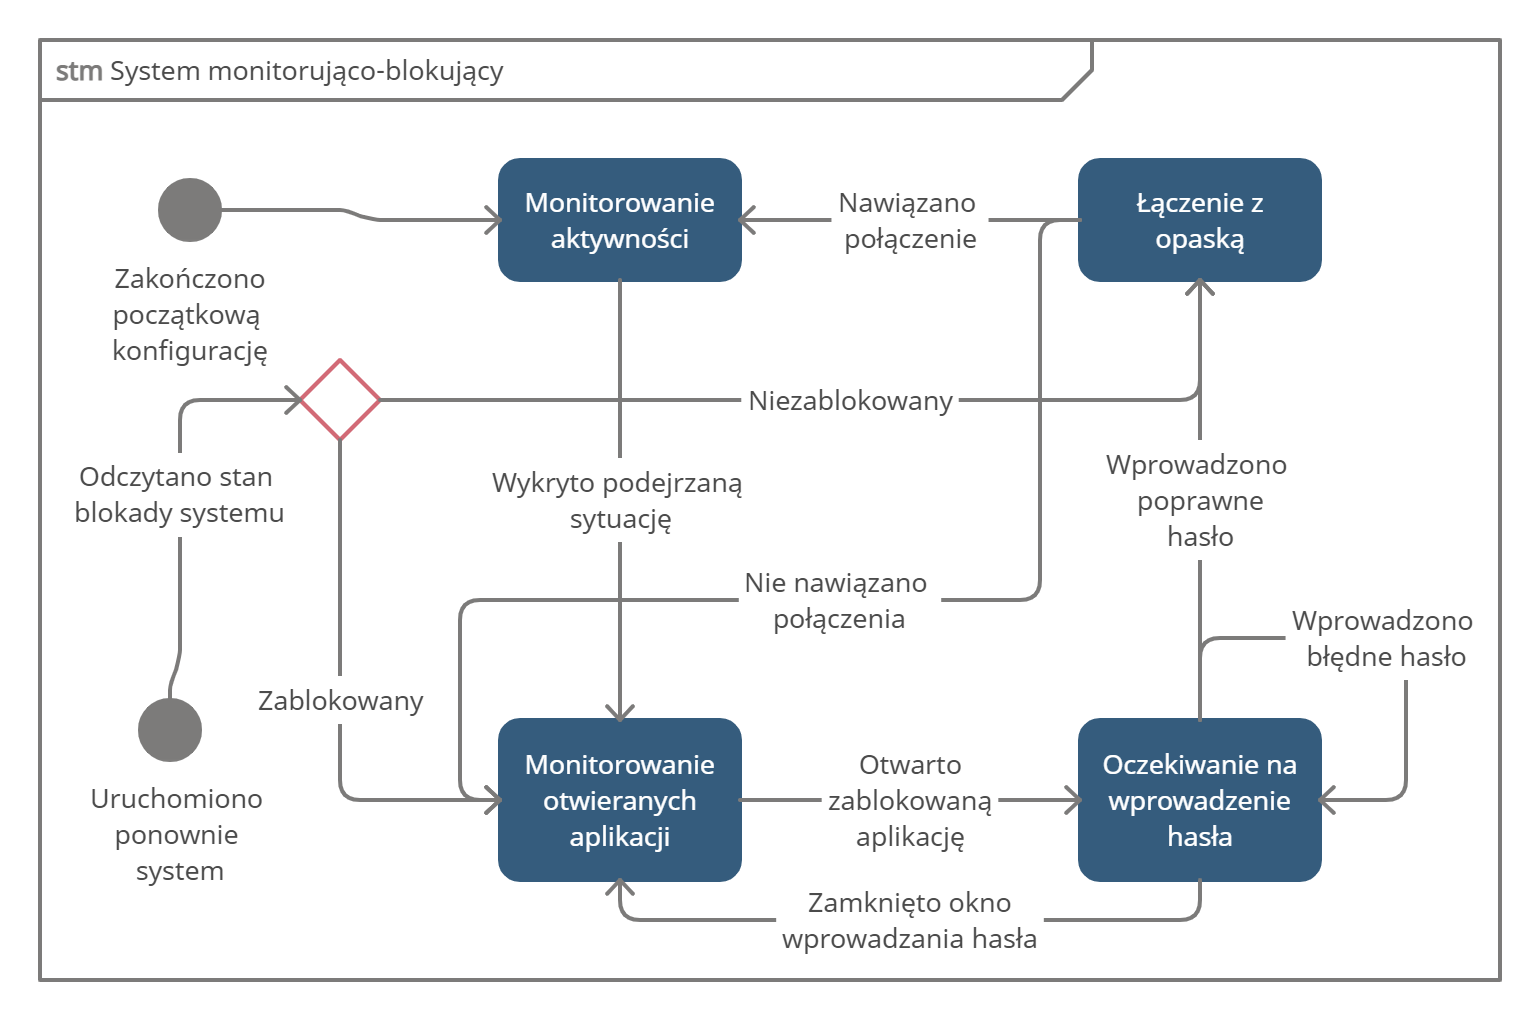
\includegraphics[width=0.9\textwidth]{MainStateDiagram.png}
    \end{center}
    \caption{{\color{dgray}Diagram stanów systemu monitorująco-blokującego.}} \label{main_state_diagram}
\end{figure}

\section{Projekt bazy danych}
Na grafice \ref{db_tables} przedstawiono tabele znajdujące się w bazie danych aplikacji. Tabele z próbkami aktywności zostały umieszczone w osobnych, niepowiązanych tabelach, by podkreślić rożnice pomiędzy rejestrowanymi rodzajami aktywności. Z kolei tabela zawierająca informacje o blokowanych aplikacjach naturalnie nie ma związku z danymi o aktywności. Proponowana aplikacja na tym stopniu zaawansowania nie wymaga bardziej skomplikowanej struktury bazy.
\newline\newline
\indent Tabela \textit{app\_states} przechowuje dane pozwalające zidentyfikować każdą zainstalowaną na smartfonie aplikację oraz wartość \textit{lock\_check}, która określa, czy dostęp do danej aplikacji będzie możliwy w czasie blokady czy nie - 0 dla dozwolonych aplikacji, a 1 dla niedozwolonych. Łańcuch znaków \textit{label} przedstawia wyświetlaną nazwę aplikacji i jest obecny w tabeli, by umożliwić przyjazne użytkownikowi wyświetlanie jej w interfejsie graficznym.
\newline\newline
\indent Tabela \textit{heart\_rate} przechowuje zarejestrowane przez opaskę informacje o pulsie wraz z czasem otrzymania danej próbki. Tabela \textit{steps\_band} posiada próbki dziennych kroków pobranych z opaski wraz z czasem ich otrzymania. Tabela \textit{steps\_phone} zawiera informacje rejestrowane przez sensor kroków w smartfonie wraz z czasem ich zapisu. Dane tej tabeli nieznacznie różnią się od danych z tabeli \textit{steps\_band}. Wartość \textit{step\_count} to liczba kroków wykonanych danego dnia, natomiast \textit{offset} jest wartością zwracaną przez sensor. Przechowywanie \textit{offsetu} jest konieczne ze względu na sposób, w jaki sensor wykorzystany w aplikacji liczy kroki - są mierzone od ostatniego restartu urządzenia. Dlatego, żeby uzyskać poprawną informację na temat dziennej liczby kroków należy monitorować zmiany w \textit{offsecie}. Wszystkie tabele z danymi o aktywności posiadają autoinkrementowane \textit{id} ze względu na to, że \textit{timestamp} nie zapewnia unikalności Primary Key.

\begin{figure}[H]
    \begin{center}
        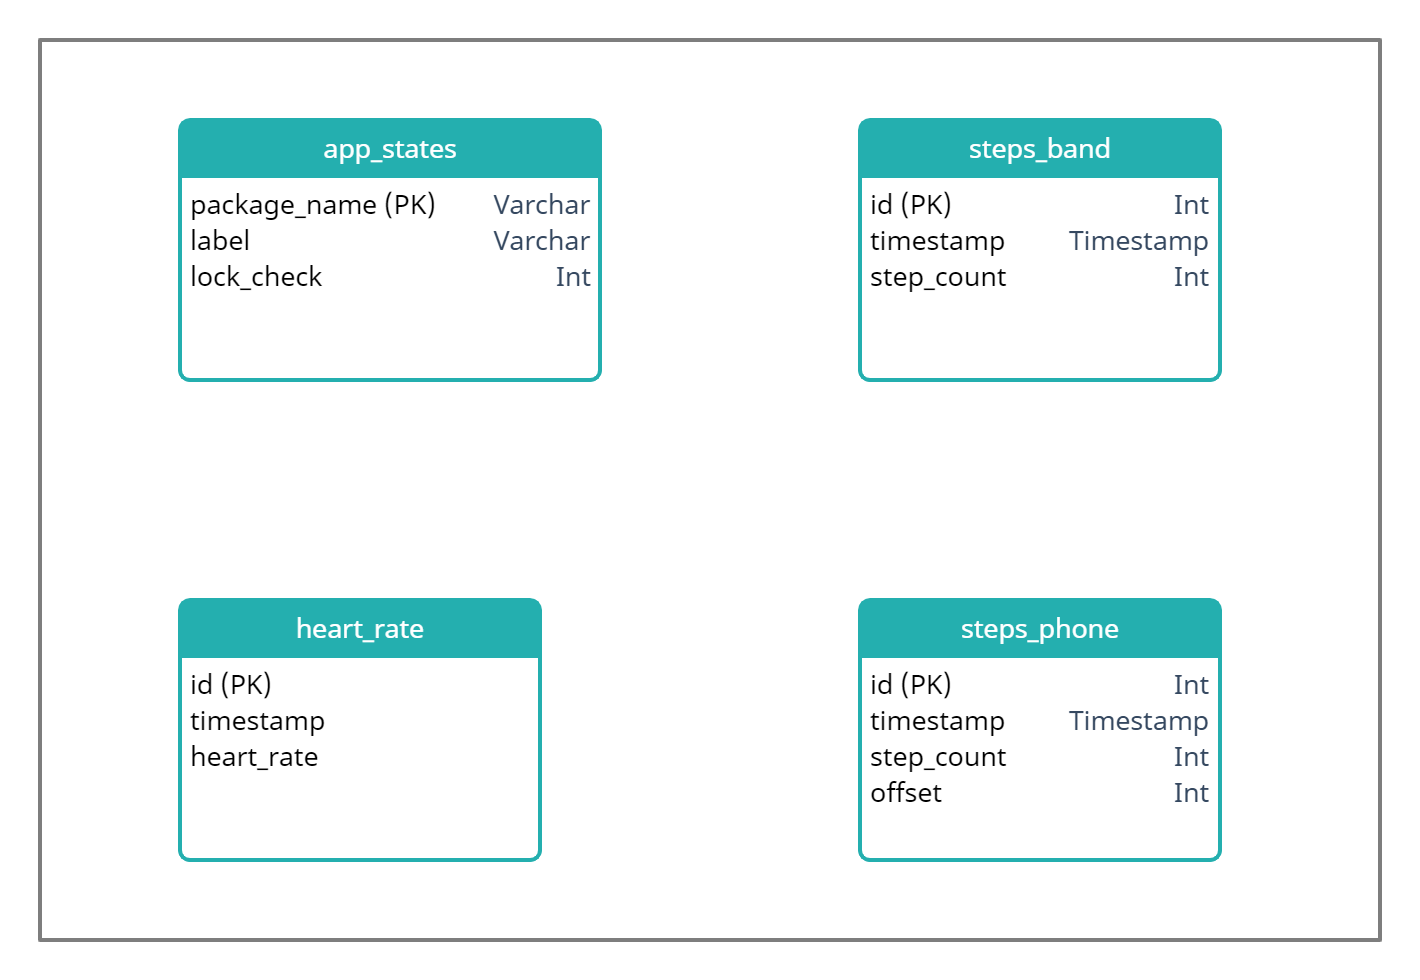
\includegraphics[width=0.9\textwidth]{DBTables.png}
    \end{center}
    \caption{{\color{dgray}Tabele w bazie danych aplikacji.}} \label{db_tables}
\end{figure}